\documentclass[a4paper,titlepage]{scrartcl}
\pagestyle{plain}
\usepackage[utf8]{inputenc}
\usepackage[T1]{fontenc}
\usepackage[german]{babel}
\usepackage{float}
\usepackage{graphicx}
\usepackage{amsmath,amssymb,amstext,mathtools}
\usepackage{enumerate}
\usepackage{units,numprint}
\usepackage{mhchem,url,tabularx}
\usepackage{braket,caption,longtable}
\renewcommand{\sc}{\textsc}

\DeclarePairedDelimiter\abs{\lvert}{\rvert}
\numberwithin{equation}{section}

\title{Magnetische Resonanz\\\normalsize 1. Überarbeitung}
\author{Genti Saliu\\Gruppe 106}
\date{Versuchstag: 10. Dezember 2014}

\begin{document}
	\begin{titlepage}
		\maketitle
		\thispagestyle{empty}
	\end{titlepage}

\newpage
\pagenumbering{roman}
\tableofcontents

\newpage
\pagenumbering{arabic}

\section{Teil I - Elektronenspinresonanz (ESR)}
\subsection{Ziel des Versuchs}
Bei der Elektronenspinresonanz lässt man eine Probe elektromagnetische Strahlung durchlaufen. Die Probe soll sich in einem Magnetfeld befinden und permanentes magnetisches Moment bzw. ungepaarte Elektronen besitzen. Im Resonanzfall absorbiert die Probe Energie und man erhält ein Spektrum, indem man die Absorption gegen die Wellenlänge der Strahlung auftragt. Dabei räpresentieren die Linien des Spektrums Übergänge zwischen Niveaus. Damit lassen sich Energieniveaus in einem Diagramm darstellen.\\ \\
In diesem Versuch werden wir das ESR-Spektrum bei verschiedenen Frequenzen der elektromagnetischen Welle beobachten, die Magnetfeldabhängigkeit der ESR, den $g$-Faktor und die Linienbreite der Probe bestimmen.
\subsection{Theoretische Grundlagen}
\subsubsection{Drehimpuls \cite{wiki:drehimpuls}}
Der Drehimpuls ist eine physikalische Erhaltungsgröße. Bei einer Kreisbewegung kann man sich den Drehimpuls im Bezug auf das Zentrum des Kreises als Pfeil vorstellen, dessen Richtung die Drehachse der Bewegung und Länge den Schwung der Drehung angibt: je länger der Pfeil, umso größer der Drehimpuls.\\ \\
Mathematisch ergibt sich der Drehimpuls $\vec{L}$ eines Massenpunktes aus dem Kreuzprodukt seines Ortsvektors $\vec{r}$ mit seinem Impuls $\vec{p}$:
\begin{equation*}
\vec{L} = \vec{r} \times \vec{p}
\end{equation*}
In diesem Versuch befassen wir uns mit dem Drehimpuls von Quantenobjekten. Dieser tritt hier in zwei Formen auf: als der aus der klassischen Mechanik von Dreh- und Kreisbewegung abgeleitete Drehimpuls, der Bahndrehimpuls, und als der nicht mit Drehbewegungen einer Masse verbundene Spindrehimpuls.
\subsubsection{Spin}
Der Spin (englisch \emph{spin} für 'Drehung') bezeichnet den Eigendrehimpuls eines Teilchens, also das Drehimpuls des Teilchens, das um sich selbst dreht. \cite{wiki:spin}\\ \\
Der Spin hat einen unveränderlichen Betrag. Es sind bisher nur Teilchen mit Spins $0 \hbar$, $\frac{1}{2} \hbar$ und $1 \hbar$ bekannt, wobei $\hbar$ das reduzierte \emph{Plancksche Wirkungsquantum} und der Zahlenfaktor die \emph{Spinquantenzahl} sind. \cite{wiki:spin}\\ \\
Die Richtungen, in der der Spin zeigt, sind ebenfalls quantisiert. Für Teilchen mit Spin $\frac{1}{2}$ gibt es nur zwei mögliche Ausrichtungen, das Teilchen kann sich rechts oder links herum drehen. Die beiden Richtungen werden mit Vorzeichen versehen und man spricht dann von positivem oder negativem Spin. Die beiden Elektronen, die sich ein Orbital teilen, unterscheiden sich immer in ihrer Spinrichtung: ein vollbesetztes Orbital besitzt nach dem Pauli Prinzip zwei Elektronen mit jeweils positivem und negativem Spin. \cite{web:spin}\\ \\
Ein geladenes Teilchen mit Spin besitzt ein magnetisches Moment. Dies wird bei vielen Experimenten ausgenutzt: beim Einstein-de-Haas-Effekt versetzt die Änderung der Richtung des Elektronenspins in einem Eisenstab diesen in eine makroskopische Drehbewegung; die Effekte der magnetischen Kernspinresonz bzw. Elektronenspinresonanz, die in diesem Versuch behandelt werden, werden zur detaillerten Untersuchungen von Materialien, Geweben und Prozessen genutzt. \cite{wiki:spin}
\subsubsection{Magnetisches Moment des Elektrons}
Das magnetische Moment ist ein Maß für die Stärke des magnetischen Dipols. Das Elektron besitzt ein magnetisches Moment, das aus seiner Spin- und ggf. Bahnbewegung resultiert.\\ \\
Das magnetische Moment des Elektronenspins $\vec{\mu_S}$ und der Bahnbewegung $\vec{\mu_L}$ sind gegeben durch
\begin{equation*}
\vec{\mu_s}=-g_S \mu_B \frac{\vec{S}}{\hbar} \quad \quad \text{und} \quad \quad \vec{\mu_L}=-g_L \mu_B \frac{\vec{L}}{\hbar}
\end{equation*}
mit $\vec{L}$ der Bahn- und $\vec{S}$ der Spindrehimpuls, $\mu_B$ das Bohr-Magneton mit $\mu_B=\frac{e \hbar}{2 m_0}$, $g_S$ bzw. $g_L$ der \emph{Landé-Faktor}, der das Verhältnis zwischen magnetischem Moment bzw. jeweils Spin- und Bahndrehimpuls angibt.\\ \\
Das gesamte magnetische Moment resultiert aus der Summe der Drehimpulse:
\begin{equation*}
\vec{\mu_J}=-g_J \mu_B \frac{\vec{J}}{\hbar}
\end{equation*}
wobei $\vec{J}=\vec{L}+\vec{S}$. Der Landesche Faktor $g$ ist gegeben durch:
\begin{equation*}
g_J=\frac{3}{2}+\frac{S (S+1) - L(L+1)}{2J(J+1)}
\end{equation*}
\subsubsection{Magnetisches Moment des Moleküls, ungepaarte Elektronen \cite{mappe}}
Beim magnetischen Moment des Moleküls kommt es auf die magnetischen Momente aller ihrer Elektronen an: der Bindungselektronen und der Elektronen in den Schalen der einzelnen Kerne.\\ \\
Elektronen in gefüllten Schalen haben einen Gesamtdrehimpuls Null. Bei zwei Bindungselektronen stehen die Spins antiparallel, der Gesamtdrehimpuls ist wiederum Null. Daher gibt es kein resultierendes magnetisches Moment und das Molekül ist diamagnetisch.\\ \\
Moleküle, die Elektrone mit fehlendem spin-kompensierendem Partner besitzen, können paramagnetisch sein. In organischen Radikalen ist das der Fall, denn diese Elektrone haben $p$-Charakter; deren magnetisches Moment kommt nur von ihren Spins, denn das Bahnmoment ist ausgelöscht. Der Paramagnetismus dieser Moleküle stammt allein aus dem magnetischen Moment dieser Elektrone.
\subsubsection{Zeeman-Effekt \cite{wiki:zeeman}}
Bringt man ein Atom mit paramagnetischen Eigenschaften in ein magnetisches Feld ein, so spalten sich seine Energieniveaus auf. Die Aufspaltung entsteht durch die Wirkung des Magnetfelds auf das magnetische Moment des Atoms $\vec{\mu_J}$:
\begin{equation*}
\vec{\mu_J}=-g \cdot \frac{\mu_B}{\hbar} \vec{J}
\end{equation*}
Man unterscheidet zwischen normalem (ohne Spindrehimpuls) und anormalem Zeeman-Effekt (mit Spindrehimpuls).
\subsubsection{Elektronenspinresonanz (ESR)}
In der Elektronenspinresonanz werden Proben mit permanentem magnetischem Moment eingesetzt. Die Paramagnetismus beruht, wie in den vorherigen Abschnitten behandelt, auf ungepaarte Elektrone. Dabei besitzt jedes Elektron bekanntlich ein magnetisches Moment mit Spinquantenzahl $s=\frac{1}{2}$ und magnetischen Komponenten $m_s=+ \frac{1}{2}$ und $m_s=-\frac{1}{2}$. Bringt man die Probe in ein statisches und homogenes Magnetfeld der Feldstärke $\vec{B}$, so richten sich die magnetischen Momente des Elektrons entweder parallel ($m_s=-\frac{1}{2}$) oder antiparallel ($m_s=+\frac{1}{2}$) zur Feldrichtung, wobei jede Ausrichtung aufgrund des Zeeman-Effekts die Energien besitzt:
\begin{equation*}
E=\frac{1}{2}g\mu_B B
\end{equation*}
Es kommt also zu einer Aufspaltung eines Energieniveaus $E_0$ mit Beteiligung des Spindrehimpulses (anormaler Zeeman-Effekt) in den Niveaus $E_1$ und $E_2$ auf (Abbildung \ref{fig:aufspaltung}).
\begin{figure}[H]
	\centering
	\begin{tabular}{@{}r@{}}
		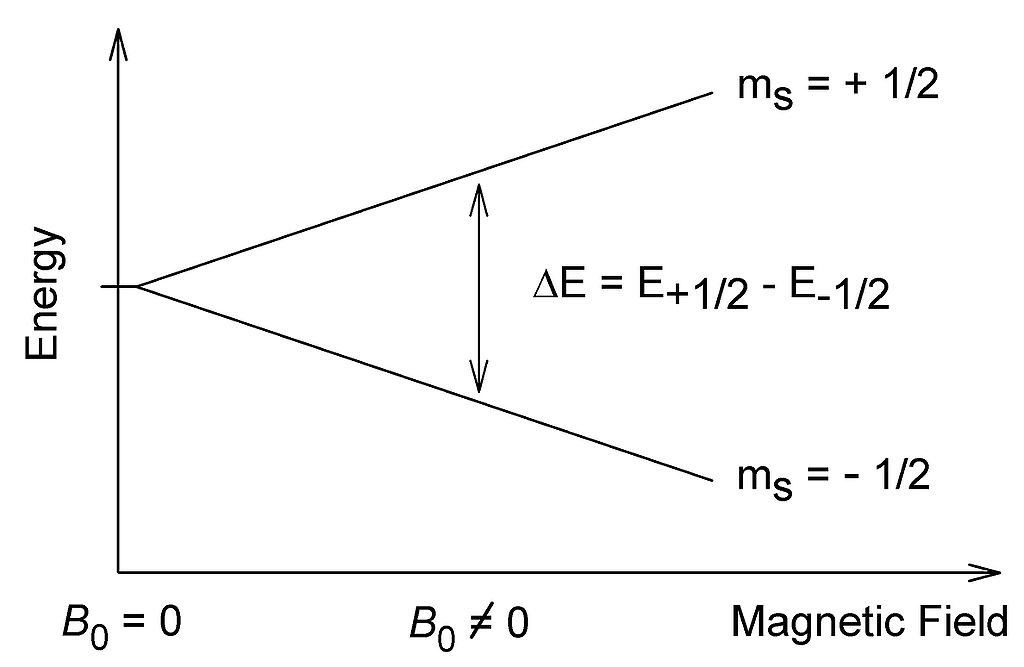
\includegraphics[width=0.5\textwidth]{images/EPR_splitting.jpg}\\
		\footnotesize\sffamily\textbf{Quelle:} Wikipedia \cite{wiki:epr}
	\end{tabular}
	\caption{Energieaufspaltung aufgrund des anormalen Zeeman-Effekts}
    \label{fig:aufspaltung}
\end{figure}
Ein ungepaartes Elektron kann zwischen diesen beiden Niveaus wechseln, wenn man eine zirkular polarisierte elektromagnetische Welle einstrahlt. Der Übergang passiert dann, wenn die eingestrahlte Welle dieselbe Energie hat, die dem Abstand zwischen der Energien der zwei Niveaus $E_1$ und $E_2$ unter Berücksichtigung der Auswahlregeln entspricht. Diesen Übergang bezeichnet mal als Elektronenspinresonanz.\cite{mappe}\\ \\
Die Resonanzbedingung bei Absorption bzw. Emission magnetischer Dipolstrahlung lautet:
\begin{equation}
\Delta E=\hbar \omega=g \mu_B \cdot B
\label{eq:resonanzBedingung}
\end{equation}
\subsubsection{Besetzungszahlen}
Die paramagnetische Substanz kann Strahlung absorbieren und emittieren. Absorption führt dazu, dass ein Elektron auf ein höheres Niveau angehoben wird, bei Emission gerät das Elektron in ein niedrigeres Niveau.\\ \\
Die Stärke der Absorption bzw. Emission hängt von der Differenz der Besetzungszahlen der Niveaus ab. Die Besetzungszahl ist die Zahl der Teilchen, die sich in einem Mikrozustand auf einem bestimmten Energieniveau befinden.\\ \\
Die Wahrscheinlichkeit, dass ein Vielteilchensystem im thermischen Gleichgewicht sich im Zustand $\ket{n}$ mit der Energie $E_n$ befindet, ist gegeben durch:
\begin{equation*}
\rho_n=const \cdot e^{-\frac{E_n}{kT}}
\end{equation*}
Den Spin des Elektrons kann man als ein System mit zwei möglichen Energiezuständen $E_1$ und $E_2$ auffassen. Damit gilt für das Verhältnis der Besetzungszahlen:
\begin{equation*}
\frac{n_2}{n_1}=e^{-\frac{E_2-E_1}{kT}}
\end{equation*}
Bezeichnet Zustand 1 den energieärmeren Zustand und Zustand 2 den energiereicheren Zustand, so gilt $\Delta E=E_2-E_1$. Da Besetzungsinversion im thermischen Gleichgewicht nicht auftritt, also dass sich mehr Teilchen in einem energetisch höheren als in einem energetisch niedrigen Zustand befinden, gilt für die Differenz der Besetzungszahlen $\Delta n=n_1-n_2$.\\ \\
Aus obiger Gleichung folgt:
\begin{equation*}
\Delta n=n \cdot \frac{1-e^{-\frac{\Delta E}{k_B T}}}{1+e^{-\frac{\Delta E}{k_B T}}}
\end{equation*}
Die Entwicklung der Exponentialfunktion im Zähler bis zur 1. Ordnung und der im Nenner bis zur 0. Ordnung nach $\Delta E$ um $\Delta E_0=0$ ergibt:
\begin{equation}
\label{eq:besetzungszahl}
\Delta n \approx n \cdot \frac{\Delta E}{2kT}=n \cdot \frac{g \mu_B B}{2 k T}
\end{equation}
Aus Gleichung \ref{eq:besetzungszahl} kann man folgende Schulussfolgerungen ziehen:
\begin{itemize}
\item Die Absorption ist proportional zur Gesamtzahl der Moleküle. 
\item Die Absorption ist proportional zur Magnetfeldstärke $B$. Ein starkes Signal erhält man also bei hohen Magnetfeldern.
\item Die Absorption ist umgekehrt proportional zur Temperatur. Messungen bei tiefen Temperaturen ergeben ein starkes ESR-Signal.
\end{itemize}
\subsubsection{Hyperfeinstruktur}
Man würde nun erwarten, dass man im ESR-Spektrum eine Einzellinie beobachtet, was normalerweise nicht der Fall ist. Die Energieniveaus werden weiter aufgespaltet. Dies hat 2 Ursachen:
\begin{itemize}
\item Ungepaarte Elektronen der paramagnetischen Substanz wechselwirken mit den magnetischen Momenten der Atomkerne des gleichen Moleküls. Dies erzeugt am Ort des Elektrons ein weiteres Magnetfeld, das sich dem äußeren überlagert.
\item Isotropie der Elemente, welche keine Aufpsaltung sondern eine Verschiebung des Spektrums verursacht \cite{wiki:hyperfeinstruktur}.
\end{itemize}
Diese Effekte nennt man zusammenfassend Hyperfeinstruktur.
\subsubsection{Auswahlregeln}
Aufgrund des Zeeman-Effekts und der Hyperfeinstruktur entstehen viele Energiniveaus. Übergänge sind nicht zwischen beliebigen Niveaus möglich, sie unterliegen den sogenannten Auswahlregeln, die nur eine Änderung um eine Einheit der magnetischen Quantenzahl des Systems und keine Änderung der Richtung des Kerndrehimpulses erlauben:
\begin{equation*}
\Delta m_s=\pm 1 \quad \quad \Delta m_I=0
\end{equation*}
\subsubsection{Linienform}
Die ESR-Resonanzlinien können unterschliedliche Formen haben: die Grenzfälle sind die Gauß- und Lorentzform:
\begin{figure}[H]
	\centering
	\begin{tabular}{@{}r@{}}
		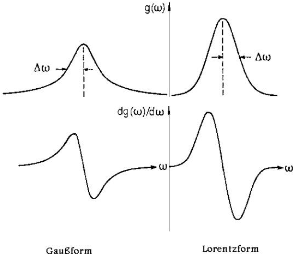
\includegraphics[width=0.5\textwidth]{images/linienform.png}\\
		\footnotesize\sffamily\textbf{Quelle:} Vorbereitungsmappe \cite{mappe}
	\end{tabular}
	\caption{Grenzfälle der Lineinform: Gauß- und Lorentzform}
    \label{fig:linienform}
\end{figure}
Die Linienbreite ist die halbe Breite der Absorption beim halben Wert des Linienmaximums.\\ \\
Sie wird von internen Magnetfeldern beeinflusst. Die Dipol-Dipol-Wechselwirkung liefert dabei den Hauptbeitrag. Diese Magnetfelder fluktuieren und ändern dabei zeitlich ihre Richtung und Stärke. Sind die Fluktuationen gegenüber der charakteristischen Zeit der Dipol-Dipol-Wechselwirkung schneller, so wird die Resonanz schmäler und Lorentzförmig, andernfalls wird sie Gaußförmig.\\ \\
Die Linienbreite wird von weiteren Faktoren beeinflusst:
\begin{description}
\item[Austauschverschmälerung] Werden die Abstände zwischen den paramagnetischen Molekülen so klein, so können Elektronen das Molekül wechseln, was sich auf die Zusatzfelder der benachbarten Dipole auswirkt. Erfolgt der Wechsel schnell, so wirkt auf das Elektron ein kleineres Zusatzfeld, was die Verbreiterung der Linie durch Dipol-Dipol-Wechselwirkung zunichte macht.
\item[Sättigungsverbreitung] Eine zu starke Einstrahlung der elektromagnetischen Welle bewirkt, dass beide möglichen Elektronenzustände gleich stark besetzt werden, was die Boltzmann-Verteilung aufhebt und sich als Sättigungsverbreiterung in der Resonanzlinie bemerkbar macht.
\item[Longitudinale Relaxationszeit $T_1$] Das ist die für eine Probe charakteristische Zeit, in der die Spin-Gitter-Relaxation erfolgt. Letztere beschreibt den Prozess, bei dem nach einem Resonanzfall, welcher das thermische Gleichgewicht der Probe und folglich die Boltzmann-Verteilung stört, diese wiederherstellt.
\item[Transversale Relaxationszeit $T_2$] Durch Einstrahlen der elektromagnetischen Welle entsteht eine rotierende Quermagnetisierung, die innerhalb der transversalen Relaxationszeit $T_2$ durch verschiedene Effekte wieder abgebaut wird. Dieses zusätzliche Magnetfeld führt ebenfalls zu einer Linienverbreiterung.
\end{description}
\subsection{Experimenteller Aufbau}
In diesem Versuch verwenden wir eine \textbf{Diphenyl-Picryl-Hydrazyl (DPPH)-Probe}, die ein ungepaartes Elektron mit stark unterdrücktem Bahndrehimpuls besitzt. Sein $g$-Faktor mit $g=2.00363$ kommt dem des freien Elektrons mit $g=2.002322$ sehr nahe. DPPH hat eine sehr schmale und intensive Resonanzlinie.\\ \\
Desweiteren wird ein \textbf{ESR-Grundgerät} verwendet. Dieses enthält einen Probenkopf, an den verschiedene Steckspulen, die verschiedene Frequenzen liefern, angebracht werden können. Sie bilden einen Schwingkreis. In den Steckspulen kann die Probe DPPH eingeschoben werden, die dort den hochfrequenten elektromagnetischen Wellen ausgesetzt wird. Die Frequenzbereiche der Spulen betragen:
\begin{itemize}
\item Spule 1: \unit[13-30]{MHz}
\item Spule 2: \unit[30-75]{MHz}
\item Spule 3: \unit[75-130]{MHz}
\end{itemize}
Am Gerät können die Frequenzen innerhalb dieser möglichen Bereiche verändert werden, die eingestellte Frequenz wird angezeigt. Es kann außerdem die Amplitude verändert werden.\\ \\
Ein passiver Schwingkreis, der für den Vorversuch nötig ist, wird auch mitgeliefert.\\ \\
Das Grundgerät wird mit Gleichspannung und einem ESR-Adapter versorgt. Das \textbf{Helmholtz-Spulenpaar}, mit Spulen vom Durchmesser $2R=\unit[13.5]{cm}$ und Windungszahl $n=320$, die in einem Abstand von $R=\unit[6.8]{cm}$ voneinander montiert sind, wird durch einen Stelltrafo mit Wechselspannung betrieben. Es erzeugt im Innenraum ein nahezu homogenes Magnetfeld:
\begin{equation}
\label{eq:esrMagnetfeld}
B=I \cdot \unit[3.96]{\frac{mT}{A}}
\end{equation}
In diesem Magnetfeld wird die Probe eingebracht, um dort die Aufspaltung der Energieniveaus durch den Zeeman-Effekt hervorzurufen.\\ \\
Es wird zudem noch ein \textbf{Oszilloskop} benötigt, um die Resonanzspektren zu beobachten. An den Kanal 1 wird die Spannung am Schwingkreis gelegt, an den Kanal 2 die Spannung, die am Helmholtz-Spulenpaar anliegt. Diese wird über einem $\unit[1.07]{\Omega}$-Widerstand abgegriffen. Wegen der Größe des Widerstandes (weil $\approx \unit[1]{\Omega}$, gilt $I[A]=U[V]$) entspricht die gemessene Spannung der Stromstärke, die durch die Helmholtz-Spulen durchfließt.
\subsection{Durchführung der Versuche}
\subsubsection{1. Versuch: Vorversuch}
Im Vorversuch sollte gezeigt werden, dass einem Hochfrequenz-Oszillator Energie entzogen wird, wenn er sich in Resonanz mit einem äußeren Schwingkreis befindet. \\ \\
Es stehen dazu der der Probenkopf am ESR-Grundgerät (hochfrequenter Oszillator), ein passiver Schwingkreis, ein Amperemeter mit $\unit[300]{\mu A}$-Messbereich und ein ESR-Betriebsgerät zur Spannungsversorgung zur Verfügung. Dabei stellt der passive Schwingkreis ein Ersatzmodell für die später einzusetzende Probe dar.\\ \\
Statt dem Betriebgsgerät, verwendeten wir im Versuch durchgehend 2 separate Spannungsquellen mit ESR-Adapter. Der Probenkopf wurde an die Spannungsquelle angeschlossen und auf eine mittlere Frequenz eingestellt. Der passive Schwingkreis wurde so gegenüber dem Probenkopf angebracht, dass die beiden Spulen sich genau gegenüber standen. Das ESR-Grundgerät wurde mit dem Amperemeter angeschlossen.\\ \\
Die Frequenz des hochfrequenten Schwingkreises wurde in kleinen Schritten variiert, bis sie mit der Resonanzfrequenz des passiven Schwingkreises übereinstimmte.\\ \\
Die Resonanzfrequenz des passiven Schwingkreises befindet sich zwischen $\unit[10]{MHz}$ und $\unit[50]{MHz}$. Deshalb wurde am Probenkopf die 2. Spule mit Frequenzbereich $\unit[30-75]{MHz}$ eingebaut. Trat Resonanz auf, so zeigte das Amperemeter einen minimalen Strom an.
\subsubsection{2. Versuch: Elektronenspinresonanz}
Der passive Schwingkreis wurde entfernt und durch die DPPH-Probe ersetzt, die möglichst in der Mitte eines Helmholtzspulenpaars eingebracht wurde. Über einen Stelltrafo, der die Spannung stets von Null bis zu einem Maximalwert durchlaufen ließ, wurde das Spulenpaar mit Spannung versorgt. Damit ändert sich auch das Magnetfeld periodisch von Null bis zu einem Maximalwert. Ein einohmiger Widerstand wurde in Reihe mit der Spule angeschlossen und, wie bereits erwähnt, die dort abfallende Spannung an den Kanal 2 des Oszilloskops gespeist.\\ \\
An den Kanal 1 legten wir die am hochfrequenten Schwingkreis anliegende Spannung. Tritt Resonanz auf, so wird dem Schwingkreis Energie entzogen und die Spannung sinkt auf einem Minimum. Auf dem Oszilloskop sollte wie in Abbildung \ref{fig:resonanz1} ein Peak (Minimum) zu sehen sein. Ist die Maximalmagnetfeldstärke größer als die Resonanzfeldstärke, so wird die Resonanz 2 mal pro Halbperiode durchlaufen, man sieht 2 Linien auf dem Schirm (Abbildung \ref{fig:resonanz2}).
\begin{figure}[H]
\centering
\begin{minipage}{.4\textwidth}
	\centering
  	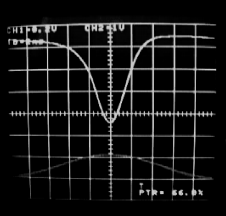
\includegraphics[width=.7\linewidth]{images/resonanz1.PNG}\\
  	\footnotesize\sffamily\textbf{Quelle:} Vorbereitungsmappe \cite{mappe}
    \captionsetup{width=0.8\textwidth}
  	\captionof{figure}{Resonanz bei maximaler Feldstärke}
  	\label{fig:resonanz1}
\end{minipage}%
\begin{minipage}{.4\textwidth}
	\centering
	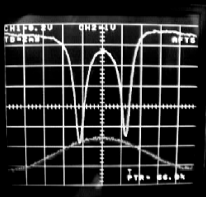
\includegraphics[width=.7\linewidth]{images/resonanz2.PNG}\\
	\footnotesize\sffamily\textbf{Quelle:} Vorbereitungsmappe \cite{mappe}
	\captionsetup{width=0.8\textwidth}
	\captionof{figure}{Resonanz wird 2 mal durchlaufen}
	\label{fig:resonanz2}
\end{minipage}
\end{figure}
Die Resonanz wurde für alle 3 Steckspulen beobachtet. Es wurde die Magnetfelstärke variiert, indem man schrittweise die Spannung des Stelltrafos $U_{Trafo}$ erhöhte. Es konnten in allen Fällen 4 Resonanzlinien festgestellt werden.\\ \\
Für Spule 2 waren die Resonanzlinien bei $U_{Trafo}\approx \unit[20-25]{V}$ zu erkennen, die Amplituden waren sehr niedrig, für Spule 3 waren sie mit höherer Amplitude bei $U_{Trafo}\approx \unit[5-25]{V}$ sichtbar und für Spule 1 im Bereich $U_{Trafo}\approx \unit[7.5-25]{V}$ mit sehr hohen Amplituden erkennbar.
\subsubsection{3. Versuch: Magnetfeldabhängigkeit der Resonanzfrequenz}
Es sollte nun die Magnetfeldabhängigkeit der Resonanzfrequenz untersucht werden. Dazu wurde die maximale Magnetfeldstärke zu einem größeren Wert als die Resonanzfeldstärke eingestellt, sodass sie doppelt während einer halben Periode auftritt. Dadurch konnten zwei ESR-Minima auf dem Display des Oszilloskops beobachtet werden.\\ \\
Dann wurde die DPPH testweise vom Probenkopf entfernt, daraufhin verschwanden die Resonanzpeaks und es waren nur die sinusförmigen Spannungsschwingungen auf dem Oszilloskop zu sehen. Damit konnte man sich überzeugen, dass die Resonanz tatsächlich durch die Probe DPPH verursacht wurde.\\ \\
Nach Wiedereinbrigen der DPPH-Probe in den Probenkopf, veränderten wir bei gleichbleibender Frequenz die Amplitude des hochfrequenten Oszillators. Je größer die Amplitude, umso höher wurden die Peaks (bzw. Amplitude) der Resonanzkurve. Das war zu erwarten, denn je größer die Amplitude der eingestrahlten Welle, umso größer die dadurch verursachte Absorption der Probe.\\ \\
Anschließend veränderten wir die magnetische Flussdichte $\vec{B}$ und stellten fest, dass eine Erniedrigung die Breite der Resonanzlinien kleiner machte, ihre Peaks liefen dabei zusammen.
\subsubsection{4. Versuch: Bestimmung des $g$-Faktors}
Nun sollte die Magnetfeldabhängigkeit der Resonanzfrequenz untersucht werden. Wir messten für verschiedene Frequenzen bei allen 3 Spulen die Resonanzen. Dazu wurde die Spannung, die am Helmholtzspulenpaar anliegt, in Abhängigkeit von der Frequenz des Schwingkreises aufgenommen.\\ \\
In der Anzeige vom Oszilloskop schwingte das Magnetfeld nicht in Phase mit der Spannung; die Peaks waren verschoben. Wir bestimmten deshalb 2 Messpunkte in der Nähe des Nulldurchgangs der Spannung, da diese in diesem Bereich annährend linear verläuft. Durch Mitteln der Beträge dieser 2 Punkte kann die Verfälschung, die diese Verschiebung verursacht, vermieden werden:
\begin{equation*}
\overline{U}=\frac{|U_{links}|+|U_{rechts}|}{2}
\end{equation*}
Die nachfolgenden Tabellen zeigen die Messdaten.
\begin{longtable}[H]{c|c|c|c}
$f$ $[MHz]$ & $U_{links}$ $[mV]$ & $U_{rechts}$ $[mV]$ & $\overline{U}$ $[mV]$ \\
\hline
$20$ & 133 & -266 & 199.5\\
$25.5$ & 183 & -316 & 249.5\\
$31$ & 233 & -366 & 299.5\\
$36.5$ & 283 & -416 & 349.5\\
$42$ & 333 & -466 & 399.5\\
$47.5$ & 400 & -533 & 466.5\\
$53$ & 450 & -566 & 508.0\\
$58.5$ & 500 & -633 & 566.5\\
$64$ & 566 & -683 & 624.5\\
$69.5$ & 616 & -733 & 674.5\\
$75$ & 683 & -783 & 733.0\\
\caption{Messreihe für die (mittlere) Spule 2}
\label{tab:spule2}
\end{longtable}
\begin{longtable}[H]{c|c|c|c}
$f$ $[MHz]$ & $U_{links}$ $[mV]$ & $U_{rechts}$ $[mV]$ & $\overline{U}$ $[mV]$ \\
\hline
$75$ & 616 & -833 & 724.5\\
$84$ & 700 & -900 & 800.0\\
$94$ & 800 & -983 & 891.5\\
$103$ & 900 & -1080 & 990.0\\
$109$ & 966 & -1130 & 1048.0\\
\caption{Messreihe für die (kleine) Spule 3}
\label{tab:spule2}
\end{longtable}
\begin{longtable}[H]{c|c|c|c}
$f$ $[MHz]$ & $U_{links}$ $[mV]$ & $U_{rechts}$ $[mV]$ & $\overline{U}$ $[mV]$ \\
\hline
$13$ & 66 & -166 & 116.0\\
$18$ & 116 & -233 & 174.5\\
$24$ & 183 & -283 & 233.0\\
$30$ & 250 & -333 & 291.5\\
\caption{Messreihe für die (große) Spule 1}
\label{tab:spule2}
\end{longtable}
\subsubsection{5. Versuch: Messung der Linienbreite}
In diesem Versuch musste die Linienbreite der Resonanzkurven bei verschiedenen Frequenzen gemessen werden. Wie bereits in den theoretischen Grundlagen eingeführt, die Breite des Resonanzpeaks bei dessen halber Höhe entspricht der Linienbreite. Dazu wurde die Spannung links und rechts des Peaks bei halber Peakhöhe bestimmt und die Differenz berechnet. Die Messung wurde nur für die (mittlere) Spule 2 durchgeführt (Tabelle \ref{tab:linienbreite}).
\begin{longtable}[H]{c|c|c|c}
$f$ $[MHz]$ & $U_{links}$ $[mV]$ & $U_{rechts}$ $[mV]$ & $\Delta U$ $[mV]$ \\
\hline
$30$ & -216 & -433 & 217\\
$52$ & -483 & -600 & 117\\
$75$ & -700 & -800 & 100\\
\caption{Messreihe zur Linienbreitenbestimmung}
\label{tab:linienbreite}
\end{longtable}
\subsection{Auswertung}
\subsubsection{Bestimmung des $g$-Faktors}
Im Resonanzfall gilt nach Gleichung \ref{eq:resonanzBedingung}:
\begin{equation*}
h \nu=g \mu_B \cdot B
\end{equation*}
Einsetzen der Magnetfeldstärke nach Gleichung \ref{eq:esrMagnetfeld} ergibt:
\begin{align}
h \nu&=g\mu_B \cdot I \cdot \unit[3.96]{\frac{mT}{A}} \Longleftrightarrow \nonumber \\
h \nu&=g\mu_B \cdot \frac{\overline{U}}{R} \cdot \unit[3.96]{\frac{mT}{A}} \Longleftrightarrow \nonumber \\
h \nu&=g \cdot \left( \frac{e \cdot h}{m_e 4 \pi} \right) \cdot \frac{\overline{U} \cdot 3.96 \cdot 10^{-3}}{\unit[1.07]{\Omega}} \frac{T}{A} \Longleftrightarrow \nonumber \\
\nu&=g \cdot \left( \frac{e \cdot \overline{U} \cdot 3.96 \cdot 10^{-3}}{m_e 4 \pi \cdot \unit[1.07]{\Omega}} \frac{T}{A} \right) \label{eq:gauswertung}
\end{align}
Der $g$-Faktor lässt sich also bestimmen, indem man die Resonanzfrequenz $\nu$ über $\frac{\mu_B B}{h}$ aufträgt und die Steigung $g$ der Regressionsgerade ermittelt. Im Folgenden wird dies für die Messreihen der einzelnen Spulen gemacht.
\begin{description}
\item[Messreihe für die (mittlere) Spule 2] Es wurde die Magnetfeldstärke bei Frequenzen $\unit[20-75]{MHz}$ gemessen. Mit linearer Regression (Abbildung \ref{fig:gmittlere}) erhielten wir folgenden Wert mit statistischem Fehler für den $g$-Faktor:
\begin{equation*}
g=1.983 \pm 0.018
\end{equation*}
\begin{figure}[H]
	\centering
	\begin{tabular}{@{}r@{}}
		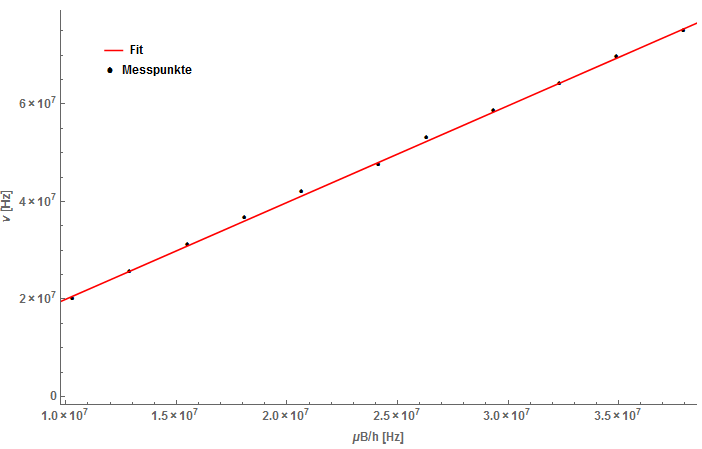
\includegraphics[width=0.8\textwidth]{images/gmittlere.png}\\
	\end{tabular}
	\caption{Bestimmung des $g$-Faktors mit der Messreihe der mittleren Spule 2}
    \label{fig:gmittlere}
\end{figure}
\item[Messreihe für die (kleine) Spule 3] Die Magnetfeldstärke wurde bei Frequenzen $\unit[70-109]{MHz}$ gemessen. Die lineare Regression der Werte (Abbildung \ref{fig:gkleine}) ergibt folgenden $g$-Wert mit statistischem Fehler:
\begin{equation*}
g=2.005 \pm 0.056
\end{equation*}
\begin{figure}[H]
	\centering
	\begin{tabular}{@{}r@{}}
		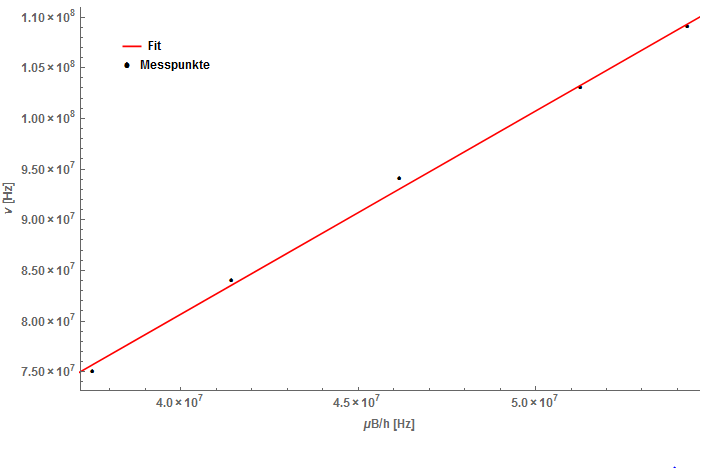
\includegraphics[width=0.8\textwidth]{images/gkleine.png}\\
	\end{tabular}
	\caption{Bestimmung des $g$-Faktors mit der Messreihe der kleinen Spule 3}
    \label{fig:gkleine}
\end{figure}
\item[Messreihe für die (große) Spule 1] Die Messung der magnetischen Feldstärke erfolgte bei Frequenzen $\unit[13-30]{MHz}$. Aus der linearen Regression der Wertepaare (Abbildung \ref{fig:ggrosse}) erhalten wir diesen $g$-Wert mit folgendem statistischen Fehler:
\begin{equation*}
g=1.881 \pm 0.057
\end{equation*}
\begin{figure}[H]
	\centering
	\begin{tabular}{@{}r@{}}
		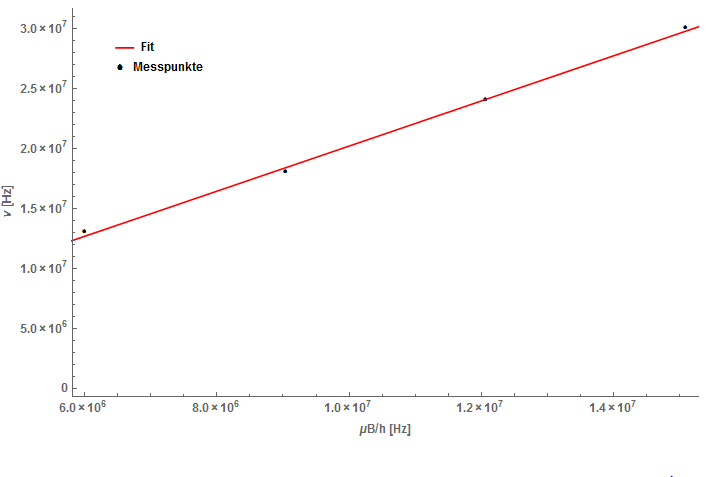
\includegraphics[width=0.8\textwidth]{images/ggrosse.png}\\
	\end{tabular}
	\caption{Bestimmung des $g$-Faktors mit der Messreihe der grossen Spule 1}
    \label{fig:ggrosse}
\end{figure}
\end{description}
Es ist nun der \textbf{systematische Fehler des $g$-Faktors} zu bestimmen. Aus Gleichung \ref{eq:gauswertung} ergibt sich der $g$-Faktor:
\begin{equation*}
g=\nu \left( \frac{m_e 4 \pi \cdot \unit[1.07]{\Omega}}{e \cdot \overline{U} \cdot \unit[3.96 \cdot 10^{-3}]{\frac{T}{A}}} \right)
\end{equation*}
Folgende Größen, von denen der $g$-Faktor abhängt, sind fehlerbehaftet:
\begin{itemize}
\item Die Frequenz $\nu$ hat einen Fehler $\sigma_{\nu}=\unit[0.05]{MHz}$, da der digitale Amperemeter sie bis zu einer Nachkommastelle angezeigt hat.
\item Die gemessene Spannung am Widerstand ist mit einem Fehler von $\sigma_{U_{Trafo}}=\unit[17]{mV}$ behaftet. Dieser Wert hängt von der Skalierung des Oszilloskops ab und wurde aus der Veränderung der Spannungsanzeige am Oszilloskopen, wenn der Cursor um einen Pixel bewegt wurde. Der $g$-Faktor wurde jedoch aus gemittelten Spannungen bestimmt:
\begin{equation*}
\overline{U}=\frac{|U_{links}| + |U_{rechts}|}{2}
\end{equation*}
Deshalb muss der Fehler der einzelnen Spannungen fortgepflanzt werden:
\begin{align*}
\sigma_{\overline{U}}&=\sqrt{\left( \frac{\partial U}{\partial |U_{links}|} \right)^2 \sigma^2_{|U_{links}|} + \left( \frac{\partial U}{\partial |U_{rechts}|} \right)^2 \sigma^2_{|U_{rechts}|}}\\
&=\frac{1}{2} \sqrt{\sigma^2_{|U_{links}|} + \sigma^2_{|U_{rechts}|}}
\end{align*}
\item Der $\unit[1.07]{\Omega}$ Widerstand wird mit einem Fehler von $\unit[2]{\%}$ angenommen. Dies entspricht einem Fehler $\sigma_R=\unit[0.0214]{\Omega}$.
\end{itemize}
Da diese Größen miteinander nicht korrelieren, kann das Fehlerfortpflanzungsgesetz angenwendet werden:
\begin{align*}
\sigma_g&=\sqrt{\left( \frac{\partial g}{\partial \nu} \right)^2 \sigma^2_{\nu} + \left( \frac{\partial g}{\partial \overline{U}} \right)^2 \sigma^2_{\overline{U}} + \left( \frac{\partial g}{\partial R} \right)^2 \sigma^2_R}\\
&=g \cdot \sqrt{\left( \frac{\sigma_{\nu}}{\nu} \right)^2 + \left( \frac{\sigma_R}{R} \right)^2 + \left( \frac{\sigma_{\overline{U}}}{\overline{U}} \right)^2}\\
&=g \cdot \sqrt{\left( \frac{\sigma_{\nu}}{\nu} \right)^2 + \left( \frac{\sigma_R}{R} \right)^2 + \frac{\sigma^2_{|U_{links}|} + \sigma^2_{|U_{rechts}|}}{4 \cdot \overline{U}^2}}
\end{align*}
Der systematische Fehler wurde für jeden Wertepaar aus den jeweiligen Messreihen der Spulen berechnet mit $m_e=\unit[9.10938291 \cdot 10^{-31}]{kg}$ und $e=\unit[1.602176565 \cdot 10^{-19}]{C}$.
\begin{itemize}
\item Systematischer Fehler der Messreihe für die (mittlere) Spule 2 
\begin{longtable}[H]{c|c|c|c}
$\nu$ $[MHz]$ & $\overline{U}$ $[mV]$ & $g$ & $\sigma_g$ \\
\hline
$20$ & 199.5 & 1.935 & 0.039\\
$25.5$ & 249.5 & 1.973 & 0.040\\
$31$ & 299.5 & 1.998 & 0.041\\
$36.5$ & 349.5 & 2.016 & 0.040\\
$42$ & 399.5 & 2.030 & 0.041\\
$47.5$ & 466.5 & 1.966 & 0.039\\
$53$ & 508 & 2.014 & 0.040\\
$58.5$ & 566.5 & 1.994 & 0.040\\
$64$ & 624.5 & 1.978 & 0.040\\
$69.5$ & 674.5 & 1.989 & 0.040\\
$75$ & 733 & 1.975 & 0.040\\
\caption{Systematischer Fehler der Messreihe für die (mittlere) Spule 2}
\label{tab:sysfehlerspule2}
\end{longtable}
Durch Mitteln der einzelnen systematischen Fehler erhalten wir den systematischen Fehler des $g$-Faktors der Messereihe zu $\sigma_{g}=0.040$.
\item Systematischer Fehler der Messreihe für die (kleine) Spule 3
\begin{longtable}[H]{c|c|c|c}
$\nu$ $[MHz]$ & $\overline{U}$ $[mV]$ & $g$ & $\sigma_g$ \\
\hline
$75$ & 724.5 & 1.998 & 0.040\\
$84$ & 800.0 & 2.027 & 0.041\\
$94$ & 891.5 & 2.036 & 0.041\\
$103$ & 990.0 & 2.009 & 0.040\\
$109$ & 1048.0 & 2.008 & 0.040\\
\caption{Systematischer Fehler der Messreihe für die (kleine) Spule 3}
\label{tab:sysfehlerspule3}
\end{longtable}
Der gemittelte systematische Fehler beträgt somit $\sigma_g=0.040$.
\item Systematischer Fehler der Messreihe für die (große) Spule 1
\begin{longtable}[H]{c|c|c|c}
$\nu$ $[MHz]$ & $\overline{U}$ $[mV]$ & $g$ & $\sigma_g$ \\
\hline
$13$ & 116.0 & 2.163 & 0.044\\
$18$ & 174.5 & 1.991 & 0.040\\
$24$ & 233.0 & 1.989 & 0.040\\
$30$ & 291.5 & 1.987 & 0.040\\
\caption{Systematischer Fehler der Messreihe für die (große) Spule 1}
\label{tab:sysfehlerspule1}
\end{longtable}
Der gemittelte systematische Fehler beträgt $\sigma_g=0.041$.
\end{itemize}
Tabelle \ref{tab:gs} fasst die Ergebnisse mit den jeweiligen systematischen und statistischen Fehlern zusammen:
\begin{longtable}[H]{cccc}
Messreihe & $g$ & Systematischer Fehler $\sigma_g$ & Statistischer Fehler $\sigma_g$ \\
\hline
Spule 1 & 1.881 & 0.041 & 0.057\\
Spule 2 & 1.983 & 0.040 & 0.018\\
Spule 3 & 2.005 & 0.040 & 0.056\\
\hline
Mittelwert & 1.956 & 0.040 & 0.044\\
\caption{$g$ Faktoren und Unsicherheiten}
\label{tab:gs}
\end{longtable}
Damit erhalten wir für den $g$-Faktor:
\begin{equation*}
\boxed{g=1.956 \pm 0.040 \pm 0.044}
\end{equation*}
\subsubsection{Linienbreite}
Die Linienbreite wurde aus dem Spannungsabstand beider Peaks bestimmt:
\begin{align}
\Delta \nu&=|\nu_1-\nu_2| \nonumber \\
&=\left| g \frac{\mu_B}{h} B_{links} \right| -\left| g \frac{\mu_B}{h} B_{rechts} \right|  \nonumber \\
&=\left| g \frac{\mu_B}{h} \frac{U_{rechts}}{R} - g \frac{\mu_B}{h} \frac{U_{links}}{R} \right| \cdot \unit[3.96]{\frac{mT}{A}} \nonumber \\
&=\left| g \frac{\mu_B}{h \cdot R} \cdot (U_{links}-U_{rechts}) \right| \cdot \unit[3.96]{\frac{mT}{A}} \nonumber \\
&=\left| g \cdot \frac{\mu_B}{h \cdot R} \cdot \Delta U \right| \cdot \unit[3.96]{\frac{mT}{A}} \label{eq:linienbreiteFormel}
\end{align}
Aus den Werten von Tabelle \ref{tab:linienbreite} auf Seite \pageref{tab:linienbreite} erhalten wir zu jeder gemessene Frequenz die Linienbreite $\Delta \nu$:
\begin{longtable}[H]{c|c|c|c}
$\nu$ $[MHz]$ & $\Delta U$ $[mV]$ & $\Delta \nu$ $[MHz]$ & $\sigma_{\Delta \nu}$ $[MHz]$ \\
\hline
$30$ & 217 & 21.986 & 2.432\\
$52$ & 117 & 11.854 & 2.432\\
$75$ & 100 & 10.132 & 2.432\\
\caption{Systematischer Fehler der Messreihe für die (kleine) Spule 3}
\label{tab:linienbreite1}
\end{longtable}
In den Rechnungen wurde der im vorherigen Abschnitt ermittelte $g=1.956$ verwendet. Die statistischen Fehler in der Tabelle wurden mit Fehlerfortpflanzung aus der Formel \ref{eq:linienbreiteFormel} für die Linienbreite berechnet:
\begin{align*}
\sigma_{\Delta \nu}&=\left( \frac{\partial \Delta \nu}{\partial (\Delta U)} \right) \sigma_{\Delta U}
\end{align*}
mit
\begin{align*}
\frac{\partial \Delta \nu}{\partial (\Delta U)}&=\frac{3.96 \cdot 10^{-3} \cdot g \cdot \mu_B}{h \cdot R}
\end{align*}
Für den Fehler $\sigma_{\Delta U}$ erhält man:
\begin{align*}
\sigma_{\Delta U}&=\sqrt{\left( \frac{\Delta U}{\partial U_{rechts}} \right)^2 \sigma^2_{U_{Traffo}} + \left( \frac{\Delta U}{\partial U_{links}} \right)^2 \sigma^2_{U_{Traffo}}}\\
&=\sqrt{2} \sigma_{U_{Traffo}}\\
&=\unit[0.024]{V}
\end{align*}
Nach Mitteln der Linienbreiten erhalten wir als Ergebnis:
\begin{equation*}
\overline{\Delta \nu}=\unit[14.658]{MHz}
\end{equation*}
Der statistische Fehler ergibt sich mit Standardabweichung zu $\sigma_{\overline{\Delta U}}=\unit[6.405]{MHz}$.\\ \\
Zusammenfassend ergibt sich für die Linienbreite mit systematischem und statistischem Fehler folgendes:
\begin{equation}
\boxed{\Delta U=\unit[14.658 \pm 0.024 \pm 6.405]{MHz}}
\end{equation}
\subsubsection{Diskussion der Ergebnisse}
Wir bestimmten den $g$-Faktor der Probe zu:
\begin{equation*}
\boxed{g=1.956 \pm 0.040 \pm 0.044}
\end{equation*}
Der berechnete Faktor entspricht sehr genau dem theoretischen Wert von $g=2.0023$ mit einer Abweichung von $\unit[2.31]{\%}$. Die Fehler sind mit $\approx \unit[4]{\%}$ gegenüber dem Wert des Faktors sehr klein. Die geringfügige Abweichung könnte mit der Inhomogenität des Feldes aus der Helmholtzspulenanordnung erklärt werden.\\ \\
Bei der Linienbreite stellt man eine zur eingestellten Frequenz umgekehrte Proportionalität fest. Der Fehler war sehr groß.
\newpage
\section{Teil II - Magnetische Kernresonanz (NMR)}
\subsection{Ziel des Versuchs}
Dieser Versuch soll die Kernspinresonanz (NMR) an Wasser und verschiedenen organischen Substanzen demonstrieren. Dabei werden deren Spektren aufgenommen und daraus die chemischen Verschiebungen, Spin-Spin-Kopplungen, Linienbreite und ggf. die molekulare Struktur der Substanzen bestimmt.
\subsection{Theoretische Grundlagen}
\subsubsection{Kernspin und magnetisches Moment}
Atomkerne besitzen ein gequanteltes Kerndrehimpuls bzw. Kernspin:
\begin{equation*}
|\vec{I}|=\hbar\sqrt{I(I+1)}
\end{equation*}
mit $I$ die Kernspinquantenzahl, die theoretisch nicht zu bestimmen ist, jedoch anhand des Schalenmodells der Kerne halb- oder ganzzahlig anzunehmen ist, und mit Planckschem Wirkungsquantum $\hbar=\unit[6.6256 \cdot 10^{-34}]{Js}$.\\ \\
Dabei ist nur die $z$-Komponente des Kernspins beobachtbar.\\ \\
Das magnetische Moment ist mit dem Drehimpuls über das gyromagnetische Verhältnis $\gamma$ verknüft:
\begin{equation*}
\vec{\mu}=\gamma \vec{I}
\end{equation*}
wobei $\gamma$ charakteristisch für jedes Isotop ist. Für den Betrag des magnetischen Moments folgt:
\begin{equation*}
|\vec{\mu}|=\gamma \sqrt{I(I+1) \hbar}
\end{equation*}
Daraus kann man ableiten, dass Kerne, für deren Kernspinquantenzahl $I=0$ gilt, keinen Drehimpuls und magnetisches Moment besitzen.
\subsubsection{Verhalten der Kerne im Magnetfeld}
Die magnetischen Dipole der Kerne der Probe sind ohne angelegtes Magnetfeld alle zufällig ausgerichtet.\\ \\
Beim Anbringen der Probe in ein starkes, statisches Magnetfeld orientieren sich die Dipole und der Drehimpuls richtet sich so aus, dass seine Komponente in Feldrichtung ein ganz- oder halbzahliges Vielfaches von $\hbar$ ist:
\begin{equation*}
I_Z=m \hbar
\end{equation*}
Dabei spalten sich die einzelnen $I_z$-Zustände aufgrund des Zeemaneffekts in verschiedene Werte der Orientierungsquantenzahl $m$, die nun Werte zwischen $-I$ und $I$ annehmen kann. Für das magnetische Moment in $z$-Richtung $\mu_z$ ergibt sich:
\begin{equation*}
\mu_z=m \gamma \hbar
\end{equation*}
Das Ausrichten der Kerne im Magnetfeld nennt man Richtungsquantelung.
\subsubsection{Kern-Zeeman-Niveaus}
Aufgrund des Zeemaneffekts, hat ein Kern hat in einem Magnetfeld der Flussdichte $B_0$ $(2I + 1)$ verschiedene Energiezustände bzw. Kern-Zeeman-Niveaus. Für die möglichen Energien erhalten wir:
\begin{equation*}
E=-\mu_zB_0=-mB_0\gamma \hbar \quad \Rightarrow \quad \Delta E=B_0 \gamma \hbar
\end{equation*}
Anhand der Boltzmann-Statistik erfahren wir, wie sich die Kerne in den verschiedenen Energieniveaus verteilen. Ist $N_b$ die Anzahl der Kerne im höher energetischen Niveau und $N_a$ die Anzahl der Kerne im niederenergetischen Niveau, so gilt:
\begin{equation*}
\frac{N_b}{N_a}=e^{-\frac{\Delta E}{k_B T}} \approx 1 - \frac{\Delta E}{k_B T}=1-\frac{\hbar B_0 \gamma}{k_B T}
\end{equation*}
Da der Energieunterschied $\Delta E$ für alle Kerne wesentlich kleiner als die mittlere Energie der Wärmebewegung $k_B T$ ist, sind alle Niveaus nahezu gleich besetzt. Der Unterschied hat die Größenordnung $10^{-6}$, wobei das energieärmere Niveau minimal bevorzugt ist.
\subsubsection{Kernresonanz}
Bestrahlt man eine sich im statischen Magnetfeld $B_0$ befindende Probe mit einer elektromagnetischen Welle einer bestimmten Frequenz $\nu_1$, so führt das für bestimmte Frequenzen dazu, dass Übergänge zwischen den verschiedenen Energieniveaus induziert werden:
\begin{equation*}
h \nu_1=\Delta E
\end{equation*}
Die Übergänge sind nur bei Erfüllung obiger Gleichung möglich. Bei Energieübergängen vom energiehöheren zum energieniedrigeren Niveau wird Energie freigesetzt, umgekehrt wird Energie absorbiert. Die beiden Vorgänge sind gleich wahrscheinlich, wobei Absorption aufgrund der stärkeren Besetzung der energieärmeren Niveaus minimal bevorzugt ist.\\ \\
Die Frequenz $\nu_1$ wird in diesem Fall Resonanzfrequenz genannt und gilt:
\begin{equation*}
\nu_1=\abs[\Big]{\frac{\Delta E}{h}}=\abs[\Big]{\frac{\gamma}{2 \pi}}B_0
\end{equation*}
Die zu $\nu_1$ gehörende Kreisfrequenz $\omega_1$ mit $\omega_1=2 \pi \nu_1$ wird ''Larmorfrequenz'' genannt.
\subsubsection{Einfluss der Umgebung des Kerns}
Da Kerne stets von Elektronen und anderen Kernen umgeben sind, müssen auch deren Einflusse auf die Resonanzen des Kernes berücksichtigt werden. Das magnetische Feld $B_{eff}$, welches auf den Kern wirkt, ist meistens kleiner als das von außen angelegte Feld $B_0$, denn die Umgebung des Kernes schirmt diesen zu einem kleinen Teil vom umgebenden Feld ab. Es gilt:
\begin{equation*}
B_{eff}=B_0-\sigma B_0=(1-\sigma)B_0
\end{equation*}
wobei $\sigma$ die Abschirmungskonstante bzw. ''chemische Verschiebung'' ist. Sie ist unabhängig vom angelegten Feld, dimensionslos und spezifisch zur elektromagnetischen Konfiguration des Kernspins und zur chemischen Umgebung des Kerns.\\ \\
Die Resonanzfrequenz $\nu_1$ verändert sich zu:
\begin{equation*}
\nu_1=\frac{\gamma}{2 \pi} (1 - \sigma) B_0
\end{equation*}
Die Resonanzfrequenz $\nu_1$ ist damit proportional zur Abschirmung $(1-\sigma)$ und zum angelegten Magnetfeld $B_0$. Das ermöglicht die Identifizierung der untersuchten Probe aus den unterschiedlichen Resonanzfrequenzen $\nu_1$.
\subsubsection{$\delta$-Skala}
Da die Resonanzfrequenz $\nu_1$ vom angelegten Magnetfeld $B_0$ abhängt, kann kein absoluter Maßstab zum Vergleich von NMR-Spektren verwendet werden. Deshalb führt man einen relativen Maßstab ein, den Frequenzunterschied $\Delta \nu$ eines NMR-Spektrums vom NMR-Spektrum einer Referenzsubstanz. Als Referenzsubstanz verwendet man Tetramethylsilan (TMS), die sich aus mehreren Gründen besonders gut geeignet ist.\\ \\
Um die Abhängigkeit des Frequenzunterschieds von der Feldstärke $B_0$ zu beseitigen, definiert man die ''chemische Verschiebung'' $\delta$:
\begin{equation}
\delta=\frac{\nu_{Probe}-\nu_{TMS}}{\nu_{TMS}} \cdot 10^6
\label{eq:deltaskala}
\end{equation}
Der $10^6$-Faktor ermöglicht die Angabe der chemischen Verschiebung in ppm (parts per million).
\subsubsection{Einfluss anderer Kerne bzw. Spin-Spin-Kopplung}
Nun müssen benachbarte Kerne berücksichtigt werden, die mit dem Kern wechselwirken. Da auch diese Spins enthalten, kommt es zu Kopplungen, sogenannt Spin-Spin-Kopplungen, die das Signal zusätzlich aufspalten. Die Kernspins polarisieren die elektronische Wellenfunktion und stehen miteinander in Wechselwirklung. Diese Aufspaltungsdifferenz wird auch indirekte Kopplungskonstante $J_{AB}$ genannt.\\ \\
Es entsteht also im Spektrum eine Feinstruktur, die nicht nur ein Singulett für die jeweilige Substanz zeigt, sondern je nach Anzahl chemisch nicht gleichwertiger Protonen in näherer Umgebung ein Dublett, Triplett, Quartett usw.\\ \\
Wir betrachten folgende Kopplungstypen:
\begin{description}
\item[Kopplung mit einem Nachbarkern]\hfill \\ Wir betrachten einen Kern A und B vom gleichen Isotop aber chemisch nicht äquivalent (besitzen unterschiedliche Resonanzfrequenzen) sind. Sie koppeln miteinander und es entsteht für jeden Kern ein Dublett, daher gibt es 4 Resonanzfrequenzen $\nu_{A1}$, $\nu_{A2}$, $\nu_{B1}$ und $\nu_{B2}$.\\ \\
Die Signalintensitäten der zwei zu einem Kern gehörenden Frequenzen sind gleich groß. Den Abstand zwischen den beiden Resonanzlinien, die zu einem Kern gehören, nennt man Kopplungskonstante $J_{AB}$. Sie ist nicht vom äußeren Feld, sondern nur vom Kernmoment abhängig.
\item[Kopplung mit zwei chemisch äquivalenten Kernen]\hfill \\ Man betrachtet einen Kern A, der zu zwei chemisch äquivalenten Kernen benachbart ist. Die Peakhöhe hängt von der Orientierung der Spins der beiden Nachbarkerne ab, dafür gibt es drei Möglichkeiten: sind beide Spins parallel bzw. antiparallel zum angelegten Feld, so wird diese verstärkt bzw. geschwächt. Sind die Spins entgegengesetzt orientiert, so heben sie sich gegenseitig auf. Es ensteht ein Triplett mit doppelter Intensität der mittleren Linie.
\item[Kopplung mit mehreren chemisch äquivalenten Kernen]\hfill \\ Das ist eine Verallgemeinerung der Kopplung mit zwei chemisch äquivalenten Kernen, der Kern ist von $n$ Kernen umgeben. Es werden $M=n+1$ Signale (Multiplett) erfasst, deren Intensitäten man nach dem Pascalschen Dreieck bestimmen kann.
\item[Kopplung zwischen nicht-äquivalenten Kernen]\hfill \\ Hier kommt es zu weiteren Aufspaltungen, beispielsweise entsteht ein Dublett eines Dubletts, denn jeder Kern wechselwirkt mit allen anderen.
\end{description}
\subsubsection{Intensität des Resonanzsignals}
Die Intensität des Resonanzsignals entspricht der Fläche unter der Absorptionssignalkurve. Sie gibt darüber Auskunft, wie viele Protone sich in einem Molekül befinden. Bei aufgespaltenen Signalen eines Multiplets muss über alle Signale integriert werden.
\subsection{Experimenteller Aufbau}
Die Kernspinresonanz wird anhand eines NMR (Nuclear Magnetic Resonance)-Spektrometers Modell EM 360-A gezeigt, das nach dem sogenannten kontinuierlichen NMR (continuous wave bzw. CW-) Verfahren arbeitet.\\ \\
Der Spektrometer besteht aus einem Radiowellensender, Magneten, Detektor, Signalverstärker und Oszilloskopen.\\ \\ 
Der Radiowellensender dient als Quelle von Radiowellen mit einstellbarer Frequenz innerhalb eines sehr schmalen Bereiches um $\unit[60]{MHz}$. Weiterhin erzeugen ein Magnet und Hilfsspulen zur Korrektur des Magnetfeldes ein konstantes $B$-Feld von $\unit[1.41]{T}$.\\ \\
Die Wellenlänge der von der Quelle ausgehenden elektromagnetischen Strahlen kann anhand der verstellbaren Frequenz angepasst werden. Diese Wellen werden über den Schwingkreis senkrecht zum magnetischen Feld eingestrahlt, wo sich eine um die $y$-Achse rotierende Probe befindet, die analog zur ESR, in eine Spule eingebracht ist (Detektor). Anhand der Spule wird die Absorption der Strahlung ermittelt, die als Spannungsausschlag über den Verstärker an das Oszilloskop übertragen wird.\\ \\
Mit dem Spektrometer sollen in diesem Versuch Wasserstoffatome detektiert werden, das Gerät ist nur dafür ausgelegt. Wasserstoff kommt am häufigsten in der Natur vor und sein Kern besteht nur aus einem Proton. Sein Gesamtkernspin beträgt $I=\frac{I}{2}$ und kann sich entweder parallel ($m=\frac{1}{2}$) oder antiparallel ($m=-\frac{1}{2}$) zur ausgezeichneten Achse einstellen. Mit dem gyromagnetischen Verhältnis ist die Nachweisempfindlichkeit eines Kernes für das NMR-Experiment verbunden. Der Wasserstoffkern besitzt ein sehr großes gyromagnetisches Verhältnis, deshalb ist er sehr gut mit dem Spektrometer zu detektieren.
\subsection{Durchführung der Versuche}
\subsubsection{Einstellen der Magnetfeldkomponenten}
Diese Aufgabe diente dazu das Magnetfeld des NMR-Gerätes einzustellen. Dies geschah mithilfe einer $\unit[8]{Hz}$-Wasserprobe bzw. ''Homo Adjust''. Die Einstellung erfolgte mit Unterstützung der Betreuerin - ein möglichst homogenes Magnetfeld sollte mit größter Sorgfalt gewählt werden, denn davon hing auch die Qualität der aufgenommenen Spektren der anderen Proben stark ab.\\ \\
Wir führten die Probe ein und stellten die Phase am Gerät ein. Die Schreiber des Oszilloskopen wurden auf die Position des maximalen Ausschlags gebracht. Wir justierten die Regler der Zusatzspulen, sodass im beobachteten Spektrum ein maximaler Ausschlag ensteht. Die Spuleneinstellungen optimierten wir solange, bis der Ausschlag nicht weiter maximiert werden konnte. Dadurch bewirkten wir eine möglichst gute Homogenisierung des Magnetfelds.\\ \\
Diese Magnetfeldeinstellungen wurden durchgehend in diesem Versuch benutzt.
\subsubsection{Aufnahme der Spektren}
Es erfolgte die Aufnahme der Spektren von Dichlormethan + Trichlormethan, \ce{C2O2H4}, \ce{C2OH6}, \ce{C2OH6}+\ce{HCL}, Isopropanol (\ce{C3OH8}) und n-Propanol (\ce{C3OH8}). Bei jeder Aufnahme wurden Phase und Feldstärke des Radiosignals neu eingestellt, um eine optimale Darstellung der Resonanzspektren zu erreichen. Die Aufnahmen dauerten alle 5 Minuten.
\subsection{Auswertung}
\subsubsection{1. Spektrum: Homo Adjust}
Wir berechnen in diesem Abschnitt die Halbwertsbreite des Wasserresonanzpeaks und vergleichen sie mit der aus der Vorbereitungsmappe (Seite 35). Aus diesem Vergleich soll sich ergeben, ob wir ein gute Auflösung bei den nächsten Messungen erreicht haben. Eine gute Auflösung bedeutet, dass das eingestellte Magnetfeld sehr homogen war.\\ \\
Die Halbwertsbreite entspricht der Breite des Resonanzsignals auf halber Ausschlagshöhe. Bei einer Ausschlagshöhe von $h=\unit[18.6]{cm}$ wurde in halber Höhe $\frac{h}{2}=\unit[9.3]{cm}$ eine Breite von $s=\unit[1.1]{cm}$ gemessen. Dabei war der Plot des Oszillographs mit $R=\unit[2]{ppm}$ skaliert, seine Gesamtbreite war $l=\unit[32.2]{cm}$. Der Skalierungsfaktor des Plots beträgt $\frac{\unit[2]{ppm}}{\unit[32.2]{cm}}=\unit[0.062]{\frac{ppm}{cm}}$ und die Breite des Peaks in ppm $\unit[0.068]{ppm}$. Der Spektrometer arbeitet bei $\unit[60]{MHz}$, was einem Wert von $\unit[4.099]{Hz}$ entspricht. Das ist in der untenstehenden Gleichung nochmal zusammengefasst:
\begin{equation*}
\sigma_{\nu_W}=\frac{R}{l} \cdot s \cdot \nu_{S}=\frac{\unit[2]{ppm}}{\unit[32.2]{cm}} \cdot \unit[1.1]{cm} \cdot \unit[60]{MHz}=\unit[4.099]{Hz}
\end{equation*}
Wir bestimmen nun den systematischen Fehler $\sigma_{\Delta_{\nu_W}}$. Die Skalierung $R$ und die Frequenz $\nu_{TMS}$ werden mit einem Fehler $\sigma_R=\unit[1]{\%}$ bzw. $\sigma_{\nu_{TMS}}=\unit[0.005]{MHz}$ angenommen, während die Fehler der Gesamtbreite $l$ und Halbwertsbreite $s$ wegen der Linienbreite des Plots $\sigma_l=\sigma_s=\unit[1]{mm}$ betragen. Das Fehlerfortpflanzungsgesetz ergibt:
\begin{align*}
\sigma_{\Delta \nu_W}&=\sqrt{\left( \frac{\partial \Delta \nu_W}{\partial R} \right)^2 \sigma^2_R + \left( \frac{\partial \Delta \nu_W}{\partial l} \right)^2 \sigma^2_l + \left( \frac{\partial \Delta \nu_W}{\partial s} \right) \sigma^2_s + \left( \frac{\partial \Delta \nu_W}{\partial \nu_{S}} \right) \sigma^2_{\nu_{TMS}}}\\ \\
&=\Delta \nu_W \sqrt{\left( \frac{\sigma_R}{R} \right)^2 + \left( \frac{\sigma_l}{l} \right)^2 + \left( \frac{\sigma_s}{s} \right)^2 + \left( \frac{\sigma_{\nu_{S}}}{\sigma_{\nu_{S}}} \right)^2}\\
&=\unit[0.375]{Hz}
\end{align*}
Mit dem Wert $\unit[4.099\pm0.375]{Hz}$ befinden wir uns deutlich unter dem aus der Vorbereitungsmappe mit $\unit[7]{Hz}$.
\subsubsection{2. Spektrum: Dichlormethan und Trichlormethan, Probe Nr. 5}
In diesem Versuch wurde eine Probe untersucht, die 2 verschiedene Substanzen enthielt, Dichlormethan \ce{CH2Cl2} und Trichlormethan \ce{CHCl3}, deren Strukturformeln jeweils den Abbildungen \ref{fig:dichlormethan} und \ref{fig:trichlormethan} entnommen werden können. Der Probe war ebenfalls TMS als Referenzsubstanz beigefügt.
\begin{figure}[H]
\centering
\begin{minipage}{.35\textwidth}
	\centering
  	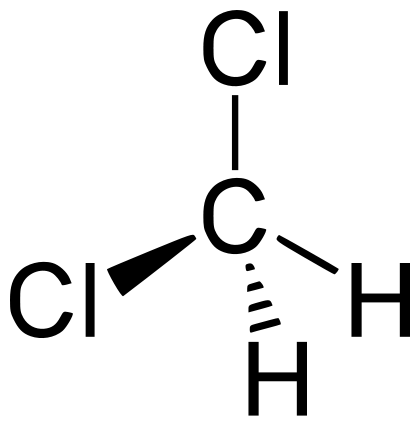
\includegraphics[width=.5\linewidth]{images/dichlormethan.png}\\
  	\footnotesize\sffamily\textbf{Quelle:} Wikipedia \cite{wiki:dichlormethan}
    \captionsetup{width=0.8\textwidth}
  	\captionof{figure}{Dichlormethan \ce{CH2Cl2}}
  	\label{fig:dichlormethan}
\end{minipage}%
\begin{minipage}{.35\textwidth}
	\centering
	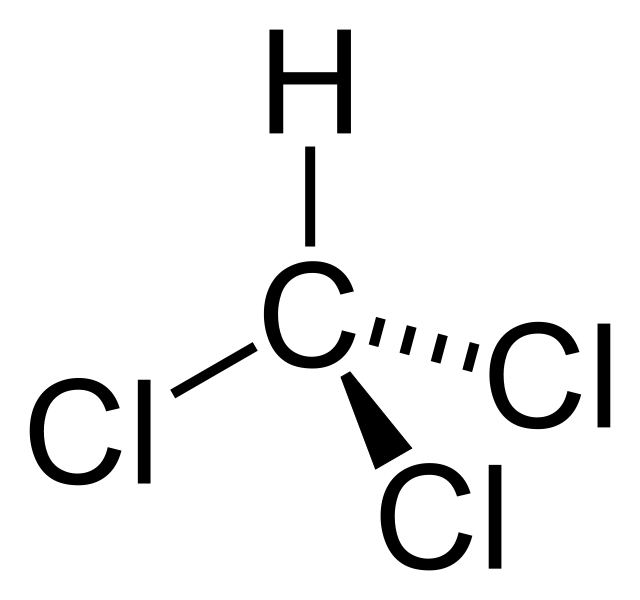
\includegraphics[width=.5\linewidth]{images/trichlormethan.png}\\
	\footnotesize\sffamily\textbf{Quelle:} Wikipedia \cite{wiki:trichlormethan}
	\captionsetup{width=0.8\textwidth}
	\captionof{figure}{Trichlormethan \ce{CHCl3}}
	\label{fig:trichlormethan}
\end{minipage}
\end{figure}
Wie man sieht, besteht Dichlormethan aus einem Wasserstofatom mehr als Trichlormethan. In beiden Substanzen kommen H-Atome vor, deshalb man 2 Resonanzpeaks zu sehen erwartet. Da \ce{CH2Cl2} doppelt so viele H-Atome als \ce{CHCl3} enthält, ist für den Peak von \ce{CH2Cl2} die doppelte Höhe zu erwarten. Beide Substanzen haben chemisch nicht-äquivalente Kerne, die im gleichen Verhältnis in der Probe vorhanden sind, weshalb es keine Aufspaltungen der Resonanzlinien gibt.\\\\
Das ist im Diagramm tatsächlich zu sehen. Ganz rechts befindet sich die Resonanzkurve von TMS, die als Referenzsubstanz verwendet wird und deren chemische Verschiebung somit $\sigma=$0 beträgt.\\ \\
Wir bestimmen nun die chemische Verschiebung $\delta$ und daraus die Linienbreite $\Delta \nu$ für die beiden Substanzen. Die chemische Verschiebung bestimmt man, indem man den Abstand der Resonanzpeaks der jeweiligen Substanzen vom TMS-Resonanzpeak im Plot misst.\\ \\
Die Plotbreite betrug $l=\unit[31.8]{cm}$, die Skalierung $R=\unit[10]{ppm}$ und die Abstände waren für:
\begin{itemize}
\item \ce{CH2Cl2}: $s=\unit[18.3]{cm}$
\item \ce{CHCl3}: $s=\unit[26.3]{cm}$
\end{itemize}
Die chemische Verschiebung in ppm bestimmen wir aus:
\begin{equation*}
\delta=\frac{s}{l} \cdot R
\end{equation*}
Den systematischen Fehler der chemischen Verschiebung $\sigma_{\delta}$ erhalten wir durch Fehlerfortpflanzung:
\begin{align}
\sigma_{\delta}&=\sqrt{\left( \frac{\partial \delta}{\partial s} \right)^2 \sigma^2_s + \left( \frac{\partial \delta}{\partial l} \right)^2 \sigma^2_l + \left( \frac{\partial \delta}{\partial R} \right)^2 \sigma^2_R} \nonumber\\
&=\frac{1}{l} \cdot \sqrt{\sigma^2_s R^2+\sigma_R l^2 + \frac{\sigma^2_l R^2 s^2}{l^2}}
\label{eq:errverschiebung}
\end{align}
Die Linienbreite $\Delta \nu$ folgt aus Gleichung \ref{eq:deltaskala}:
\begin{equation*}
\Delta \nu=\delta \cdot \nu_{TMS}
\end{equation*}
mit $\nu_{TMS}=\unit[60]{Hz}$. Daraus erhält man durch Fehlerfortpflanzung den systematischen Fehler:
\begin{align}
\sigma_{\Delta \nu}&=\sqrt{\left (\frac{\partial \Delta \nu}{\partial \delta} \right)^2 \sigma^2_{\delta} + \left( \frac{\partial \Delta \nu}{\partial \nu_{TMS}} \right)^2 \sigma^2_{\nu_{TMS}}} \nonumber \\
&=\sqrt{\nu^2_{TMS} \cdot \sigma^2_{\delta} + \delta^2 \cdot \sigma^2_{\nu_{TMS}}} \label{eq:errorfunterschied}
\end{align}
Die Breite bei halber Höhe für \ce{CH_2Cl_2} bzw. \ce{CHCl_3} beträgt für beide $\unit[3.5]{mm}$. Wir erhalten:
\begin{table}[H]
\centering
\begin{tabular}{c|c|c|c|c}
Atomgruppe & Abstand $s$ [cm] & $\delta$ [ppm] & Breite [mm] & $\Delta \nu$ [Hz]\\
\hline
\ce{CH2Cl2} & 18.3 & $5.755 \pm 0.105$ & 3.5 & $6.604 \pm 1.888$\\
\ce{CHCl3} & 26.3 & $8.270 \pm 0.105$ & 3.5 & $6.604 \pm 1.888$\\
\end{tabular}
\end{table}
\subsubsection{3. Spektrum: \ce{C2O2H4}, Probe Nr. 1}
Essigsäure besteht aus 2 Atomgruppen (\ce{CH3-COOH}, Abbildung \ref{fig:essigsaeure}), ihre Kerne sind chemisch nicht-äquivalent, wechselwirken aber nicht miteinander und die Resonanzlinien werden daher nicht aufgespalten. Es sollen also nur zwei einzelne Resonanzsignale zu sehen im Diagramm, was auch durch unsere Aufnahme bestätigt wird.
\begin{figure}[H]
	\centering
	\begin{tabular}{@{}r@{}}
		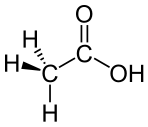
\includegraphics[width=0.2\textwidth]{images/essigsaeure.png}\\
	\footnotesize\sffamily\textbf{Quelle:} Wikipedia \cite{wiki:essigsaeure}
	\end{tabular}
	\caption{Essigsäure \ce{C2O2H4}}
    \label{fig:essigsaeure}
\end{figure}
In der \ce{CH3}-Gruppe sind drei Mal so viele H-Atome vorhanden als in den \ce{COOH}-Gruppe, deswegen sehen wir auch einen viel höheren Peak. Der Probe lag auch TMS bei, sein Peak befindet sich rechts im Plot und ist sehr klein im Vergleich zu den anderen.\\ \\
Die Skalierung des Plots betrug $R=\unit[20]{ppm}$ mit einer Gesamtbreite von $l=\unit[32.2]{cm}$. Die Messung der Abstände der Peaks der beiden Atomgruppen aus dem TMS Peak ergab die chemische Verschiebung $\delta$:
\begin{table}[H]
\centering
\begin{tabular}{c|c|c|c|c}
Atomgruppe & Abstand $s$ [cm] & $\delta$ [ppm] & Breite [mm] & $\Delta \nu$ [Hz]\\
\hline
\ce{CH3} & 3.8 & $2.360 \pm 0.209$ & 2 & $7.453 \pm 3.727$\\
\ce{COOH} & 19.3 & $11.987 \pm 0.209$ & 2 & $7.453 \pm 3.727$\\
\end{tabular}
\end{table}
\subsubsection{4. Spektrum: \ce{C2OH6}, Probe Nr. 2}
Ethanol (Abbildung \ref{fig:ethanol}) besteht aus 3 Atomgruppen bzw. 3 verschiedenen H-Kernen: \ce{CH3-CH2-OH}. Diese Kerne wechselwirken:
\begin{itemize}
\item Die \ce{CH3}-Gruppe kommt zu Wechselwirkungen mit den 2 Protonen aus der \ce{CH2}-Gruppe - es entsteht eine dreifache Aufspaltung.
\item Die \ce{CH2}-Gruppe wechselwirkt mit den 3 Protonen aus der \ce{CH3}- und wird von der \ce{OH}-Gruppe noch einmal aufgespaltet. Es sollte deshalb ein Quartett zu sehen sein.
\item Die \ce{OH}-Gruppe wechselwirkt mit den 2 Protonen aus der \ce{CH2}-Gruppe. Es ist ein Triplett zu erwarten.
\end{itemize}
\begin{figure}[H]
	\centering
	\begin{tabular}{@{}r@{}}
		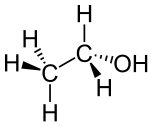
\includegraphics[width=0.2\textwidth]{images/ethanol.png}\\
	\footnotesize\sffamily\textbf{Quelle:} Wikipedia \cite{wiki:ethanol}
	\end{tabular}
	\caption{Ethanol \ce{C2OH6}}
    \label{fig:ethanol}
\end{figure}
Die Probe enthielt außer Ethanol auch TMS. \\ \\
Leider waren einige Resonanzpeaks im aufgenommenen Diagramm nicht so scharf. Die erwarteten Tripplets bei den Resonanzlinien von \ce{CH3} waren relativ gut zu erkennen, bei der \ce{CH2}-Gruppe war kein Quartett sichtbar, offensichtlich weil die Gruppe nicht mit der \ce{OH}-Gruppe wechselwirkt und deshalb zu keiner weiteren Aufspaltung kommt. Das liegt vermutlich an der Alterung der Probe. Aus dem gleichen Grund wurde bei der \ce{OH}-Gruppe kein Triplett festgestellt.\\ \\
Der Plot wurde mit $R=\unit[10]{ppm}$ skaliert und war $\unit[32.1]{cm}$ breit. Aus den gemessenen Abständen bestimmten wir für jede Atomgruppe die chemische Verschiebung $\delta$:
\begin{table}[H]
\centering
\begin{tabular}{c|c|c|c|c}
Atomgruppe & Abstand $s$ [cm] &  $\delta$ [ppm] & Breite [mm] & $\Delta \nu$ [Hz]\\
\hline
\ce{CH3} & 4.1 & $1.277 \pm 0.105$ & 1.2 & $2.243 \pm 1.869$\\
\ce{CH2} & 12.4 & $3.863 \pm 0.105$ & 1.5 & $2.804 \pm 1.869$\\
\ce{OH} & 18.4 & $5.732 \pm 0.105$ & 2 & $3.738 \pm 1.869$\\
\end{tabular}
\end{table}
Es wurden die Kupplungskonstanten $J$ für die Atomgruppen bestimmt, bei denen im Plot Aufspaltungen erkennbar waren. Die Kupplungskonstante $J$ ist der Abstand in ppm bzw. Hz zwischen der einzelnen Peaks bei Mehrfachaufspaltungen. Dabei berechnet sich der systematische Fehler der Kuplungskonstante in ppm bzw. Hz mit den Formeln \ref{eq:errverschiebung} bzw. \ref{eq:errorfunterschied}.
\begin{table}[H]
\centering
\begin{tabular}{c|c|c|c}
Atomgruppe & Abstand $s$ [cm] &  $J$ [ppm] & $J$ [Hz]\\
\hline
\ce{CH3} & 0.35 & $0.109 \pm 0.105$ & $6.540 \pm 6.300$\\
\ce{CH2} & 0.40 & $0.125 \pm 0.105$ & $7.500 \pm 6.300$
\end{tabular}
\end{table}
\subsubsection{5. Spektrum: \ce{C2OH6}+\ce{HCl}, Probe Nr. 8}
Nun wurde der vorherigen Probe Säure \ce{HCl} hinzugefügt. Es sind die gleichen Resonanzkurven zu erwarten mit dem Unterschied, dass der \ce{OH}-Peak verschwunden sein soll. Der Grund besteht darin, dass die \ce{OH}-Gruppe, aufgrund der chemischen Reaktion des Ethanols mit der Säure, aus der als Nenbenprodukt Wasser entsteht, entfernt wird. Stattdessen sollte der durch den H-Atom der Säure verursachte Peak zu sehen sein. Die zusätzliche Aufspaltung der \ce{CH2}-Gruppe, die aus \ce{OH} verursacht wurde, sollte auch verschwunden sein.\\ \\
Diese bestätigt unsere Aufnahme sehr gut, die Resonanzlinie von \ce{HCl} ist sehr scharf und hoch, was an den Mengenverhältnissen der einzelnen Substanzen liegen soll. Die Probe enthielt auch TMS.\\ \\
Der Plot war wieder mit $R=\unit[10]{ppm}$ skaliert und $l=\unit[32.1]{cm}$ breit. Der TMS-Peak war dabei zu sehen. Es wurden chemische Verschiebung $\delta$ und Linienbreite $\Delta \nu$ bestimmt:
\begin{table}[H]
\centering
\begin{tabular}{c|c|c|c|c}
Atomgruppe & Abstand $s$ [cm] &  $\delta$ [ppm] & Breite [cm] & $\Delta \nu$ [Hz]\\
\hline
\ce{CH3} & 2.1 & $0.654 \pm 0.105$ & 6.2 & $11.589 \pm 1.873$\\
\ce{CH2} & 10.8 & $3.364 \pm 0.105$ & 8.0 & $14.953 \pm 1.875$\\
\ce{HCl} & 23.4 & $7.290 \pm 0.105$ & 4.0 & $7.477 \pm 1.871$\\
\end{tabular}
\end{table}
Vergleicht man die oben bestimmte chemische Verschiebung mit der aus der Probe ohne \ce{HCL}, so weichen die Werte auch unter Berücksichtigung der Fehlergrenzen voneinander stark ab. Wir erklären das mit der Ungenauigkeit des Messgeräts, das im Verlauf der Versuchsdurchführung oft für die gleiche Probe bei verschiedenen Messungen unterschiedliche Diagramme lieferte.\\ \\
Für die jeweiligen Kopplungskonstanten $J$ ergeben sich:
\begin{table}[H]
\centering
\begin{tabular}{c|c|c|c}
Atomgruppe & Abstand $s$ [cm] &  $J$ [ppm] & $J$ [Hz]\\
\hline
\ce{CH3} & 0.40 & $0.125 \pm 0.105$ & $7.500 \pm 6.300$\\
\ce{CH2} & 0.40 & $0.125 \pm 0.105$ & $7.500 \pm 6.300$
\end{tabular}
\end{table}
\subsubsection{6. Spektrum: Isopropanol \ce{C3OH8}, Probe Nr. 3}
Isopropanol (\ce{CH3-CH-OH-CH3}, Abbildung \ref{fig:isopropanol}) besteht aus drei Atomgruppen, für die folgende Resonanzkurven zu sehen sein sollten:
\begin{itemize}
\item \ce{CH3}: diese beiden Gruppen wechselwirken nur mit der \ce{CH}-Gruppe, es wird eine zweifache Aufspaltung (Dublett) erwartet. Aufgrund der hohen Anzahl der gleichartigen beteiligten Kerne (6) soll auch der Peak im Vergleich zu den anderen Peaks hoch sein.
\item \ce{CH}: es sollte zu einer siebenfachen Aufspaltung kommen, denn die Protonen der beiden \ce{CH3}-Gruppen beeinflussen diese Gruppe.
\item \ce{OH}: es werden 2 Resonanzlinien aufgrund der Wechselwirkung mit der benachbarten \ce{CH}-Gruppe erwartet.
\end{itemize}
\begin{figure}[H]
	\centering
	\begin{tabular}{@{}r@{}}
		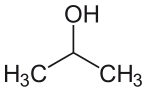
\includegraphics[width=0.2\textwidth]{images/isopropanol.png}\\
	\footnotesize\sffamily\textbf{Quelle:} Wikipedia \cite{wiki:isopropanol}
	\end{tabular}
	\caption{Isopropanol \ce{C3OH8}}
    \label{fig:isopropanol}
\end{figure}
Der aufgenommene Plot ist schlecht. Es sind zwar die 2 Aufspaltungen der \ce{CH3}-Gruppe zu sehen, jedoch sind die erwarteten Resonanzkurven für die Gruppen \ce{CH} und \ce{OH} sehr unscharf, sodass man die Aufspaltungen nicht erkennen kann. Ausserdem enthält das Spektrum Artefakte und Spiegelpeaks, die auf das Rotieren der Probe im Magnetfeld zurückgeführt werden könnten.\\ \\
Die Probe enthielt diesmal kein TMS, sodass die chemische Verschiebung anhand der TMS-Resonanzlinie aus den vorherigen Plots bestimmt wurde. Die Skalierung des Plots betrug $R=\unit[10]{ppm}$, seine Breite $l=\unit[32.2]{cm}$. Damit konnten chemische Verschiebung $\delta$ und Linienbreite $\Delta \nu$ bestimmt werden:
\begin{table}[H]
\centering
\begin{tabular}{c|c|c|c|c}
Atomgruppe & Abstand $s$ [cm] &  $\delta$ [ppm] & Breite [mm] & $\Delta \nu$ [Hz]\\
\hline
\ce{CH3} & 3.8 & $1.180 \pm 0.105$ & 6.5 & $12.112 \pm 1.867$\\
\ce{CH} & 13.2 & $4.099 \pm 0.105$ & 8.5 & $15.839 \pm 1.870$\\
\ce{OH} & 16.4 & $5.093 \pm 0.105$ & 5.0 & $9.317 \pm 1.866$\\
\end{tabular}
\end{table}
Die Kopplungskonstanten für die erkennbaren Aufspaltungen sind:
\begin{table}[H]
\centering
\begin{tabular}{c|c|c|c}
Atomgruppe & Abstand $s$ [cm] &  $J$ [ppm] & $J$ [Hz]\\
\hline
\ce{CH3} & 0.35 & $0.109 \pm 0.105$ & $6.540 \pm 6.300$
\end{tabular}
\end{table}
\subsubsection{7. Spektrum: n-Propanol \ce{C3OH8}, Probe Nr. 9}
n-Propanol (\ce{CH3-CH2^1-CH2^1-OH}, Abbildung \ref{fig:npropanol}) besteht aus 4 Atomgruppen, für die folgende Resonanzlinien zu erwarten sind:
\begin{itemize}
\item \ce{CH3} wird wegen der zwei Protonen der benachbarten \ce{CH2}-Gruppe in ein Triplett aufgespalten. Wegen der vielen H-Atomen soll auch die Höhe des Peaks groß sein.
\item \ce{CH2^2} ist mit \ce{CH3} sowie mit \ce{CH2} benachbart, seine Resonanzlinie sollte deshalb in ein Sextett aufgespaltet sein.
\item \ce{CH2^1}: die Resonanzlinie sollte sich aufgrund der zwei Protonen aus der Nachbar-\ce{CH2^2}- und dem einen Proton aus der \ce{OH}-Gruppe in ein Quartett aufspalten.
\item \ce{OH}: es wurde eine Triplettaufspaltung erwartet, aufgrund der 2 zwei Protonen aus der Nachbar-\ce{CH2^1}-Gruppe.
\end{itemize}
\begin{figure}[H]
	\centering
	\begin{tabular}{@{}r@{}}
		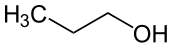
\includegraphics[width=0.2\textwidth]{images/npropanol.png}\\
	\footnotesize\sffamily\textbf{Quelle:} Wikipedia \cite{wiki:npropanol}
	\end{tabular}
	\caption{n-Propanol \ce{C3OH8}}
    \label{fig:npropanol}
\end{figure}
Unsere Aufnahme war wieder schlecht, obwohl sie mehrmals wiederholt wurde. Bei der \ce{CH3}-Resonanzlinie konnte statt dem erwarteten Triplett nur ein Dublett festgestellt werden bzw. eine Aufspaltung war stark unterdrückt. Auch der für \ce{CH2^2} erwartete Sextet konnte nicht nachgewiesen werden, dafür nur ein Quartett. Für \ce{CH2^1} konnte nur ein Triplett und vermutlich noch ein anderer unterdrückter Peak statt dem zu erwarteten Quartett erkannt werden. Die Resonanzlinie der \ce{OH}-Gruppe bestand aus einem einzelnen scharfen Peak statt in ein Triplett aufgespaltet zu sein; offensichtlich hängt das damit zusammen, dass es zu keiner Wechselwirkung dieser Gruppe mit den Nachbarn kommt.\\ \\
Ausserdem enthielt unsere Aufzeichnung viele Spiegelpeaks, die aus der Drehung der Probe im Magnetfeld verursacht sein könnten. Der Plot war mit $R=\unit[10]{ppm}$ skaliert und $l=\unit[32.1]{cm}$ breit. Es wurden chemische Verschiebung $\delta$ und Linienbreite $\Delta \nu$ bestimmt. Die Probe enthielt wieder kein TMS, sodass die Verschiebung anhand der TMS-Resonanzlinien aus früheren Aufnahmen bei gleicher Skalierung erfolgte:
\begin{table}[H]
\centering
\begin{tabular}{c|c|c|c|c}
Atomgruppe & Abstand $s$ [cm] &  $\delta$ [ppm] & Breite [mm] & $\Delta \nu$ [Hz]\\
\hline
\ce{CH3} & 5.8 & $1.807 \pm 0.105$ & 7.5 & $14.019 \pm 1.874$\\
\ce{CH2} & 7.7 & $2.399 \pm 0.105$ & 9.5 & $17.757 \pm 1.878$\\
\ce{CH2} & 14.8 & $4.596 \pm 0.105$ & 6.0 & $11.215 \pm 1.873$\\
\ce{OH} & 20.0 & $6.211 \pm 0.105$ & 3.0 & $5.607 \pm 1.870$\\
\end{tabular}
\end{table}
Die Kopplungskonstanten der Aufspaltungen der jeweiligen Resonanzlinien betragen:
\begin{table}[H]
\centering
\begin{tabular}{c|c|c|c}
Atomgruppe & Abstand $s$ [cm] &  $J$ [ppm] & $J$ [Hz]\\
\hline
\ce{CH3} & 0.2 & $0.062 \pm 0.105$ & $3.738 \pm 6.300$\\
\ce{CH2} & 0.35 & $0.109 \pm 0.105$ & $6.540 \pm 6.300$\\
\ce{CH2} & 0.3 & $0.093 \pm 0.105$ & $5.607 \pm 6.300$
\end{tabular}
\end{table}
\subsubsection{Diskussion der Ergebnisse}
Es konnte anhand der \ce{^1H}-NMR-Spektroskopie tatsächlich die molekulare Struktur der Proben bestimmt werden. Damit lassen sich an der Höhe der Peaks bzw. Anzahl der Aufspaltungen nicht nur die Anzahl der \ce{^1H}-Atome bestimmen, sondern auch die Unterscheidung der Strukturen von Substanzen ist möglich, wie das am Beispiel von Iso- und n-Propanol sehr gut klar wird, wo beide die gleiche Summenformel besitzen.\\ \\
Die meisten aufgenommenen Spektren entsprachen den (theoretischen) Erwartungen, lediglich die Spektren von Iso- und n-Propanol waren ungenau. Auch waren die berechneten chemischen Verschiebungen $\delta$ und Linienbreite $\Delta \nu$ den in der Vorbereitungsmappe aufgeführten Werten sehr nahe.\\ \\
Das Gerät war nicht immer zuverlässig - in den meisten Fällen mussten Spektrenaufnahmen mehrmals wiederholt werden.
\section{Änderungsprotokoll}
\begin{table}[H]
\centering
\begin{tabularx}{\textwidth}{| c | X |}
\hline
\textbf{Datum} & \textbf{Änderungen}\\
\hline
21. Januar 2015 & 1. Fassung\\
\hline
02. März 2015 & Teil 1 - Elektronenspinresonanz (ESR): Theoretische Grundlagen, experimenteller Aufbau und Durchführung der Versuche überarbeitet, in der Auswertung wurden im 4. Versuch Beträge statt Spannungswerte gemittelt, darauf aufbauende Berechnungen wurden korrigiert, die Linienbreite wurde in der Einheit Hertz statt Volt umgerechnet, Abschnitt zur Diskussion der Ergebnisse wurde entsprechend den neuen Erkenntnissen überarbeitet. Teil 2 - Magnetische Kernresonanz: Verbesserung mancher Formulierungen in der Vorbereitung und Auswertung, die Linienbreiten wurden berechnet\\
\hline
\end{tabularx}
\end{table}
\bibliographystyle{acm}
\bibliography{literatur}

\end{document}